\appendix
%
% If you only have one appendix, you should change the above to:
%\appendix
%
 

\chapter{DISPERSED TRAJECTORY FIGURES}

Given here are histograms showing the distribution of various performance variables relating to the vacuum and atmospheric conditions for a powered landing and descent under APDG as described in Chapters\:\ref{chap:simulation} and\:\ref{chap:results}.

\begin{figure}[H]
	\centering
	\begin{minipage}{4.3 in}
		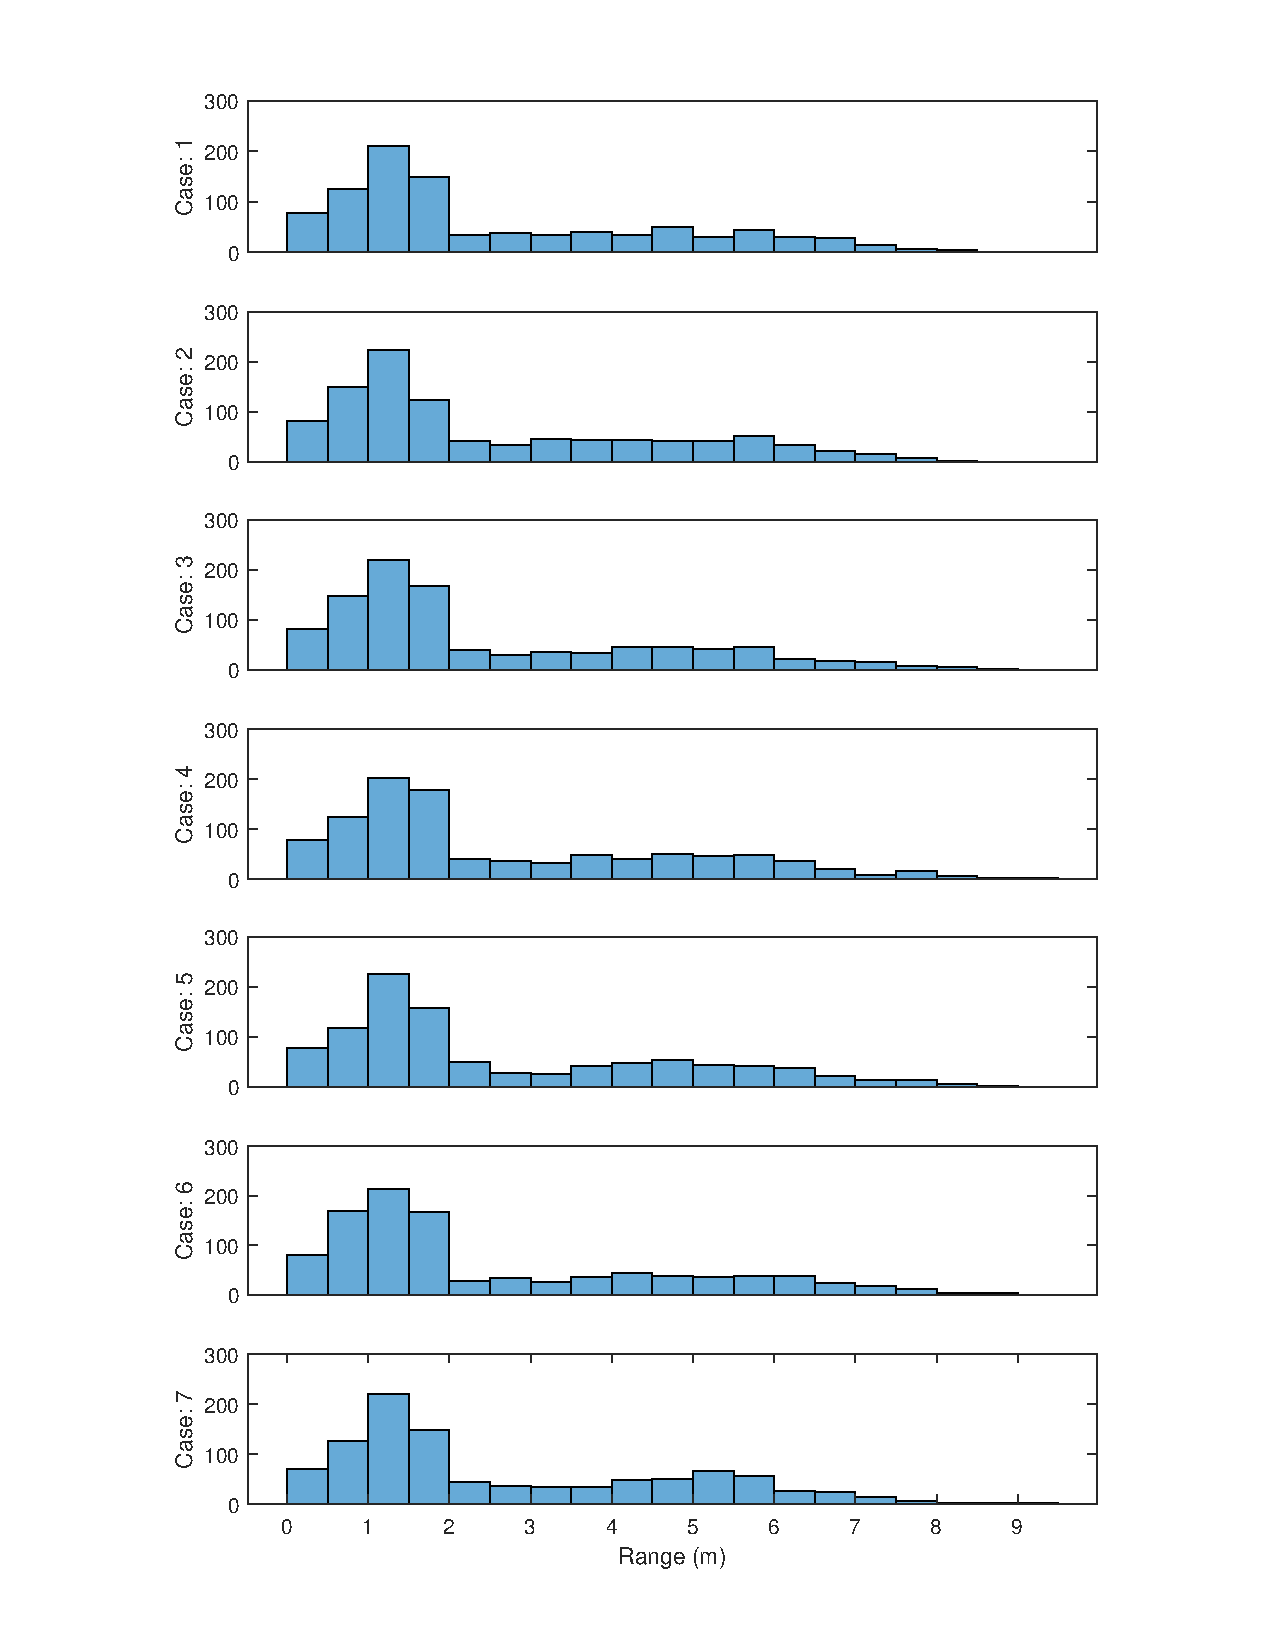
\includegraphics[width=\linewidth]{Figures/hrngdisppowvac.pdf}
		\caption{Ground Range Histogram: APDG in Vacuum \label{fig:hrngdisppowvac} }
	\end{minipage}
\end{figure}



\begin{figure}[H]
	\centering
	\begin{minipage}{4.3 in}
		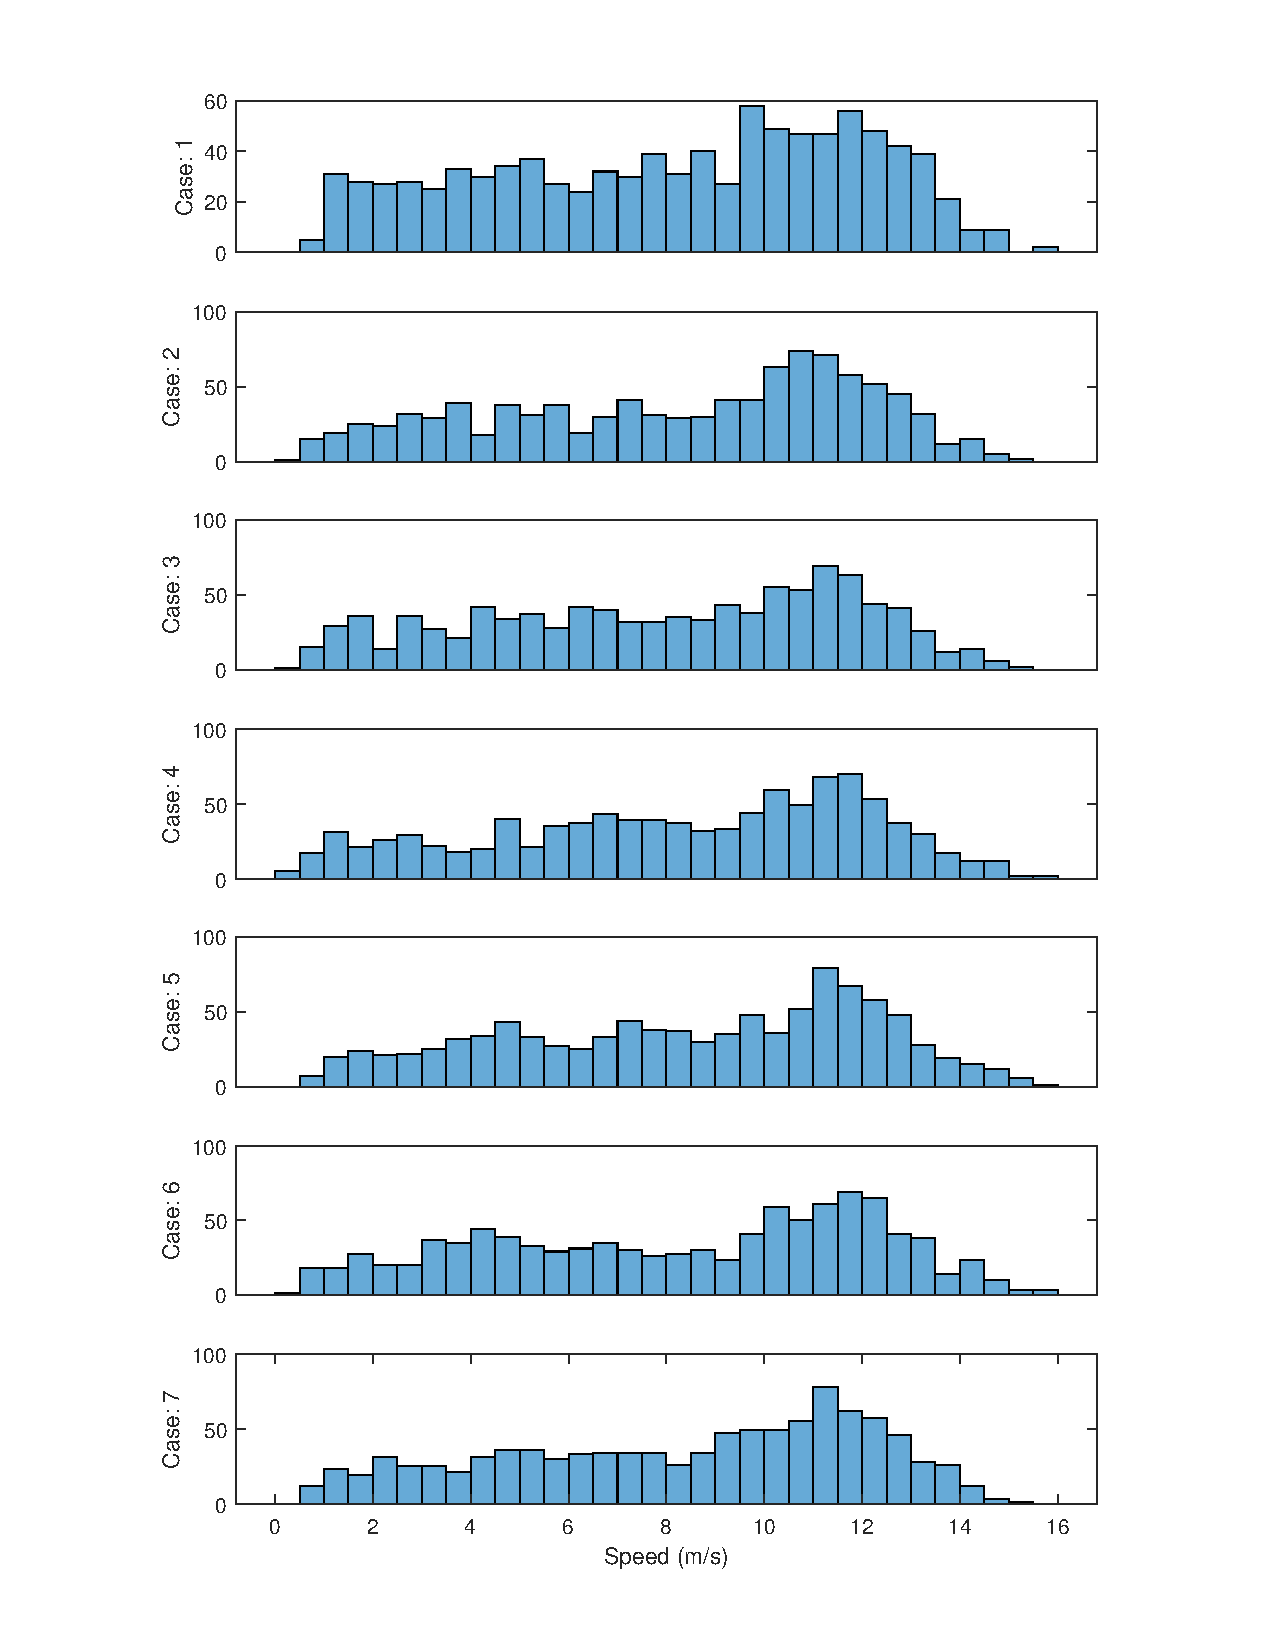
\includegraphics[width=\linewidth]{Figures/hspddisppowvac.pdf}
		\caption{Speed Histogram: APDG in Vacuum \label{fig:hspddisppowvac} }
	\end{minipage}
\end{figure}

\begin{figure}[H]
	\centering
	\begin{minipage}{4.3 in}
		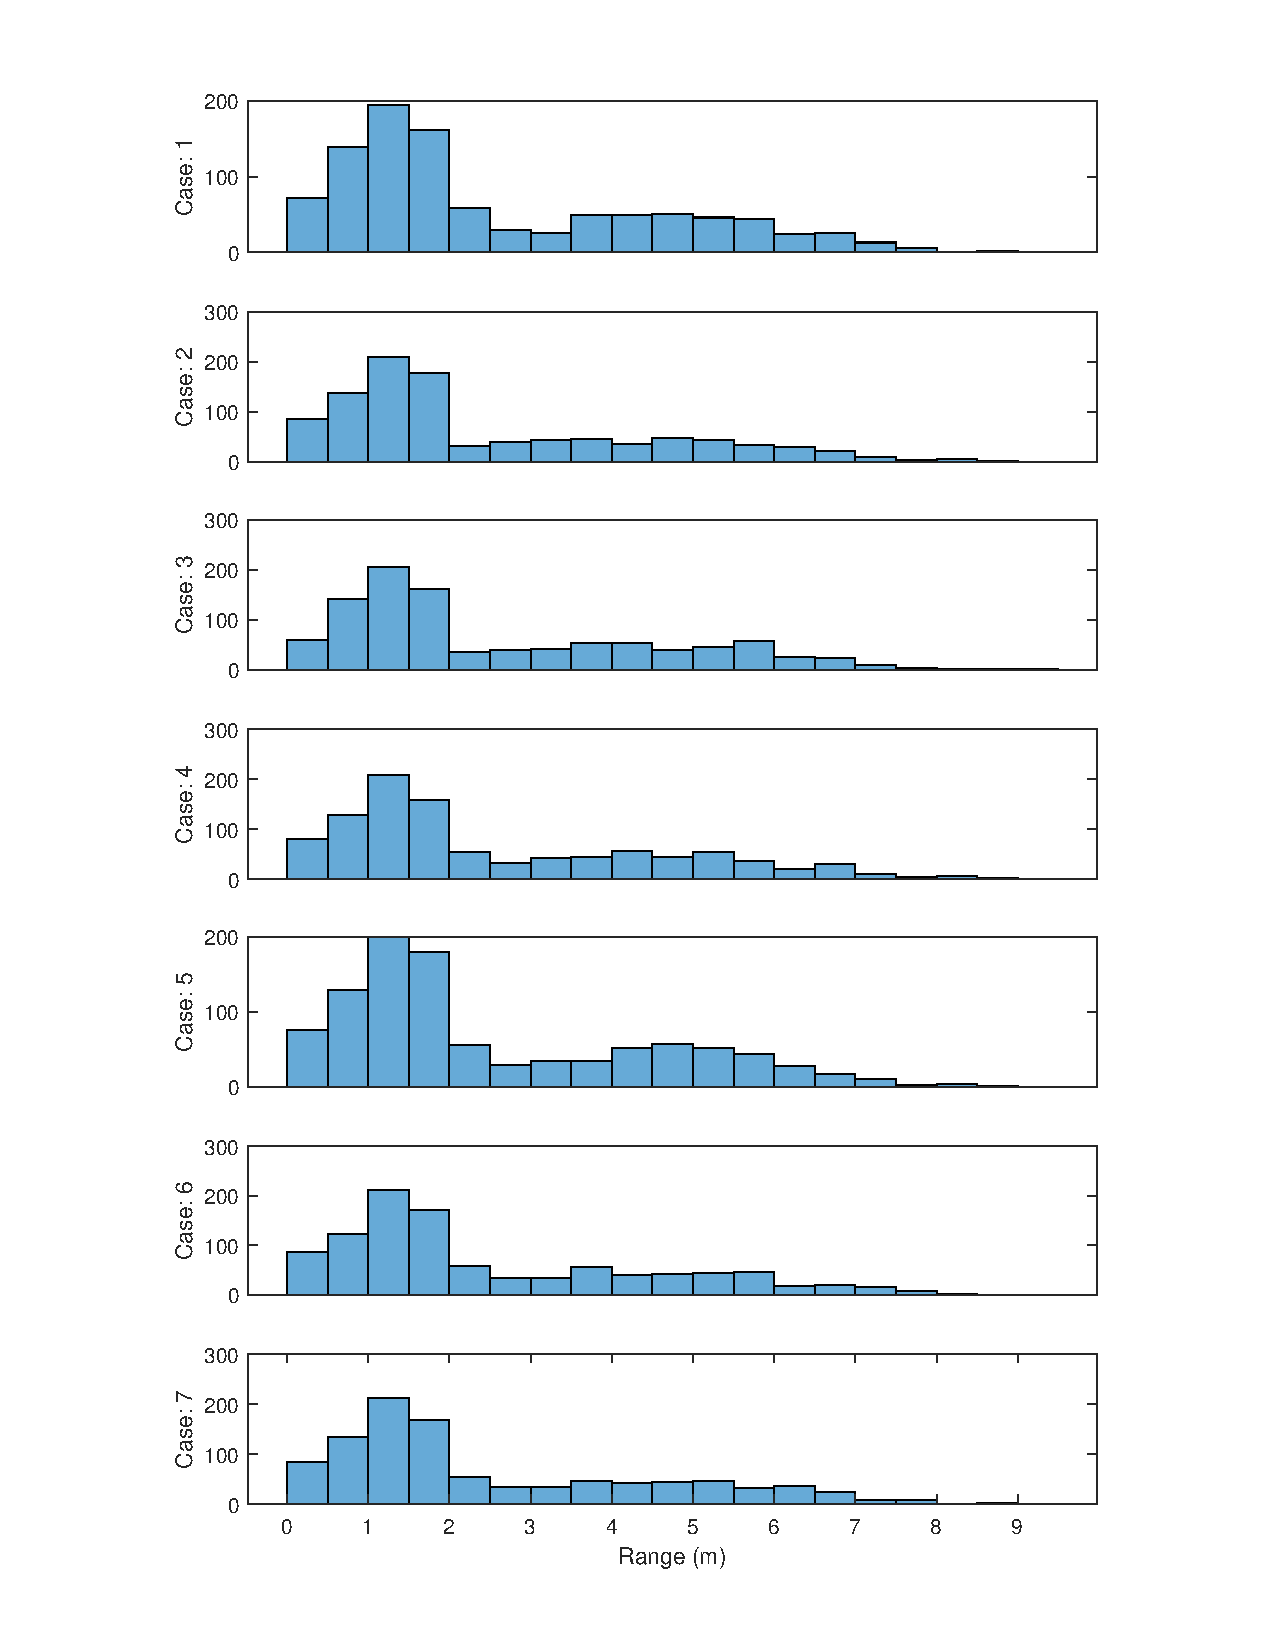
\includegraphics[width=\linewidth]{Figures/hrngdisppowatmo.pdf}
		\caption{Ground Range Histogram: APDG in Atmosphere \label{fig:hrngdisppowatmo} }
	\end{minipage}
\end{figure}



\begin{figure}[H]
	\centering
	\begin{minipage}{4.3 in}
		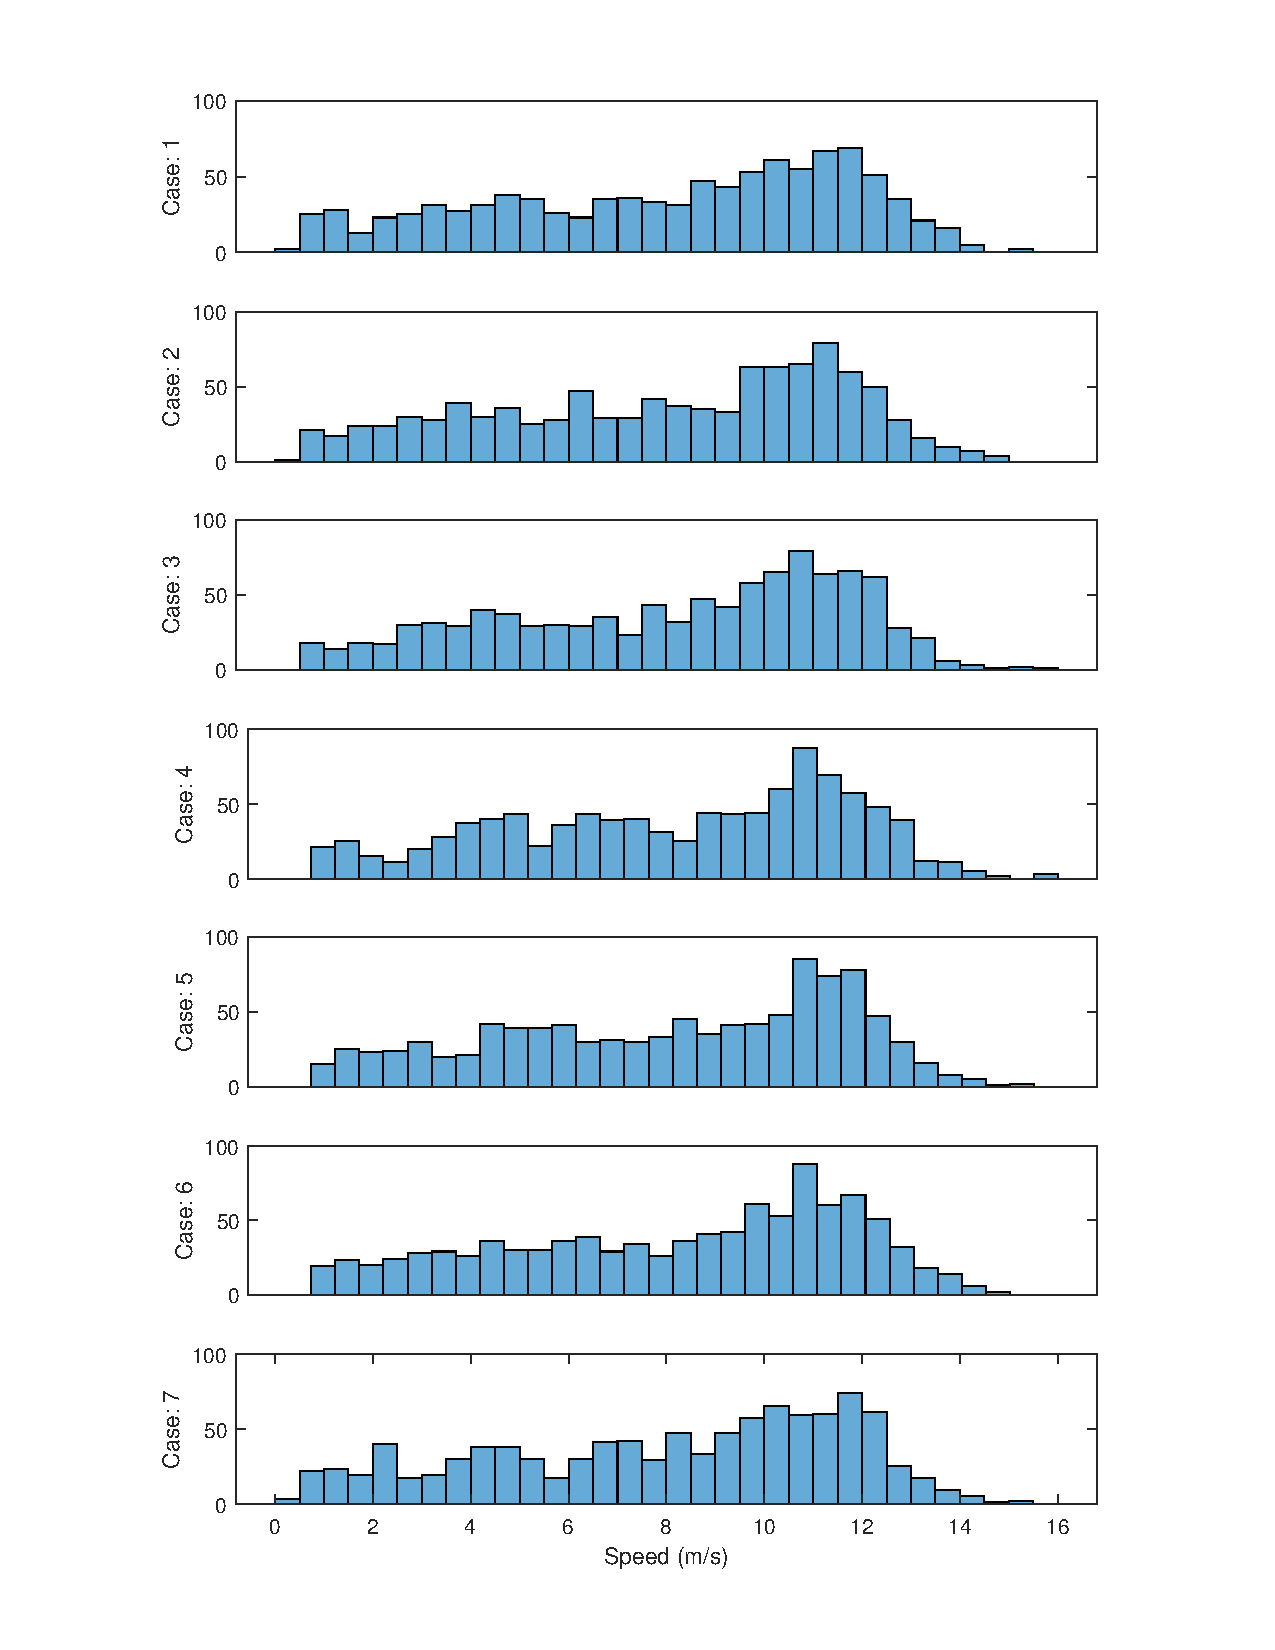
\includegraphics[width=\linewidth]{Figures/hspddisppowatmo.pdf}
		\caption{Speed Histogram: APDG in Atmosphere \label{fig:hspddisppowatmo} }
	\end{minipage}
\end{figure}



\begin{figure}[H]
	\centering
	\begin{minipage}{4.3 in}
		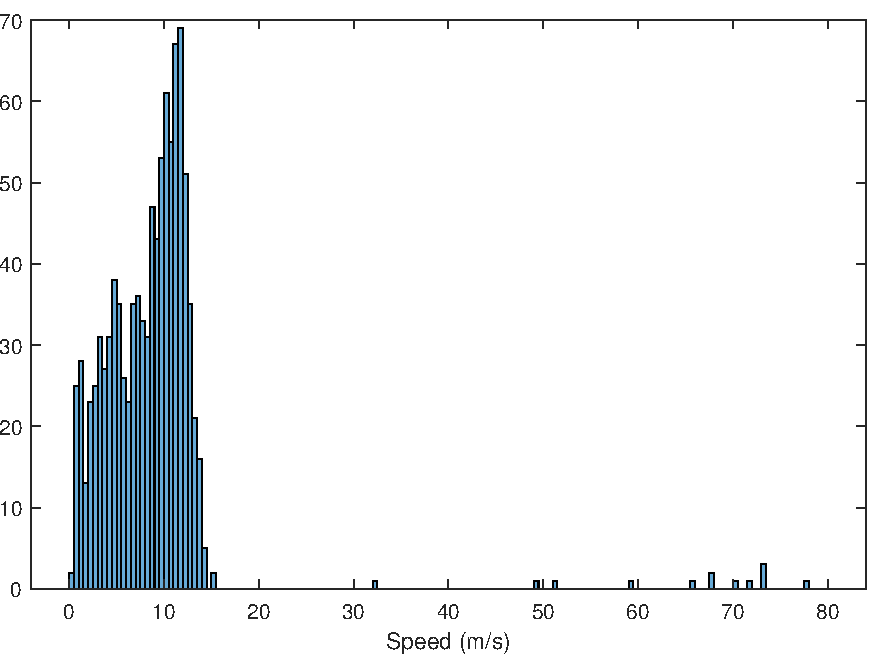
\includegraphics[width=\linewidth]{Figures/hspdfaildisppowatmo.pdf}
		\caption{Failures Histogram: APDG in Atmosphere \label{fig:hspdfaildisppowatmo} }
	\end{minipage}
\end{figure}

%To demonstrate how an appendix should be inserted into the thesis we
%have provided two appendices. This first appendix illustrates some
%more advanced techniques to improve the appearance of your equations.
%Below is a system of partial differential equations from a model for
%cellular control by an external nutrient. The equations are
%complicated and \LaTeX\ tends to allow them to run into each other. To
%prevent this we have used the \verb+\vrule+ command to separate
%them. Note this is an ordinary \TeX\ command and is not in L.\
%Lamport's book \cite{LAM}. Furthermore, we have some complicated
%boundary conditions that we needed to align, so we used the array
%command, but to get the equations looking right we also needed the
%\verb+\dfrac+ command instead of the \verb+\frac+ command. The
%equations for our model are as follows:
%\begin{eqnarray}
%  \dot{U}_1(t) & = & \tilde f(W_1(t-T)) - U_1(t) + \gamma_1U_2(R\sigma,
%   t){\vrule width 0in depth .1in},	\nonumber \\
%  \dot{W}_1(t) & = & -\hat b_3W_1(t) + \gamma_3W_2(R\sigma,
%   t){\vrule width 0in depth .1in},\nonumber \\
%  \frac{\partial U_2}{\partial t} & = & D_1\nabla^2U_2 - U_2 - \tilde f(W_1
%    (t-T)) - \gamma_1U_2(R\sigma,t){\vrule width 0in depth .1in},
%	\label{sys2} \\
%  \frac{\partial V_2}{\partial t} & = & D_2\nabla^2V_2 - b_2V_2 + c_0
%    \bigl(U_2 + U_1(t)\bigr){\vrule width 0in depth .1in}, \nonumber \\
%  \frac{\partial W_2}{\partial t} & = & D_3\nabla^2W_2 - b_3W_2 + (\hat b_3
%    -b_3)W_1 - \gamma_3W_2(R\sigma,t) \nonumber \\
%    &  & + k\left[\left[{\left(\frac{D_3}{r^2}\right)}\frac{d}{dr}\left(r^2
%	   \frac{dh}{dr}\right) - b_3h\right]V_2(R,t) - h\dot V_2(R,t)
%	   \right], \nonumber
%\end{eqnarray}
%for $t > 0$ and $R\sigma < r < R$ and with the boundary conditions:
%\begin{equation*}
%\begin{array}{rclcrcl}
% \dfrac{\partial U_2(R\sigma,t)}{\partial r} & = &
%   \beta_1U_2(R\sigma,t), & \qquad &
% \dfrac{\partial U_2(R,t)}{\partial r} & = &
%   0, \\
%\\
% \dfrac{\partial V_2(R\sigma,t)}{\partial r} & = &
%   0, & \qquad &
% \dfrac{\partial V_2(R,t)}{\partial r} & = &
%   0, \\
%\\
% \dfrac{\partial W_2(R\sigma,t)}{\partial r} & = &
%   \beta_3W_2(R\sigma,t), & \qquad &
% \dfrac{\partial W_2(R,t)}{\partial r} & = &
%   0.
%\end{array}
%\end{equation*}
%Notice that the system is numbered only once by (\ref{sys2}) and that
%this is centered as best we can on one line. All other lines have the
%$\backslash$\textit{nonumber} command.
%
%\section{Theorems}
%The appendix can also include technical theorems and lemmas which are
%call in the same manner as before. For example,
%\begin{theorem}
%  The system of equations \textrm{(\ref{sys2})} can exhibit periodic
%  solutions for certain parameter values.
%\end{theorem}
%
%\noindent
%\begin{proof}
%  The argument uses Hopf bifurcation techniques and is
%  very complicated. See Mahaffy \textit{et al} \cite{MJV}.
%\end{proof}



%The thesis will rarely use list environments, but they are valuable
%for r{\'e}sum{\'e}s. For more information on creating a r{\'e}sum{\'e}
%you may want to see the author of this document (you also need to
%learn quite a bit about \verb+\parbox+ commands).  To create a list
%you will want to use one of \texttt{itemize, enumerate,} or
%\texttt{description}. For example:
%\begin{description}
%\item[continuous] A function $f$ is {\bf continuous} at $x$ if and only
%if for every $\varepsilon >0$ there exists a $\delta(x) >0$ such that
%whenever $|y-x|<\delta$, $|f(y)-f(x)| < \varepsilon$.
%\item[uniformily continuous] A function $f$ is {\bf uniformly
%continuous} if and only if for every $\varepsilon >0$ there exists a
%$\delta >0$ such that whenever $|y-x|<\delta$, $|f(y)-f(x)| <
%\varepsilon$ independent of $x$ and $y$.
%\item[equicontinuous] A family of functions $f_n$ is {\bf
%equicontinuous} at a point $x$ if and only if for every $\varepsilon >0$
%there exists a $\delta >0$ such that whenever $|y-x|<\delta$,
%$|f_n(y)-f_n(x)| < \varepsilon$ for all functions $f_n$.
%\end{description}
%
%\LaTeX\ provides an environment for block quotations. To agree with the
%thesis manual follow the format below for a quotation exceeding four
%lines. From Lewis Carrol's {\it Hunting of the Snark} we hear the
%Bellman tell his crew:
% \vspace{.12pt}
%
%{
%\ssp
%\begin{verse}
%The Bellman himself they all praised to the skies--\\
%Such a carriage, such ease and such grace!\\
%Such solemnity, too! One could see he was wise,\\
%The moment one looked in his face!\\
% \vspace{.15in}
%He had bought a large map representing the sea,\\
%Without the least vestige of land:\\
%And the crew were much pleased when they found it to be\\
%A map they could all understand.\\
% \vspace{.15in}
%``What's the good of Mercator's, North Poles and Equators,\\
%Tropics, Zones, and Meridian Lines?''\\
%So the Bellman would cry: and the crew would reply,\\
%``They are merely conventional signs!''\\
% \vspace{.15in}
%``Other maps are such shapes, with their islands and capes!\\
%But we've got our brave Captain to thank''\\
%(So the crew would protest) ``that he's bought us the best--\\
%A perfect and absolute blank!''\\
%\end{verse}
%}
%
